\svnInfo $Id$


% --------------------------------------------------------------------------------
\section{Available output fields}\label{nest:sec_outfields}
% --------------------------------------------------------------------------------

\begin{table}[t]
  \centering
  \begin{tabular}{|p{5cm}|p{4.5cm}|p{4.5cm}|}\hline
    \rowcolor{Gray}
                               &    {\centering\textbf{global lat-lon}}          &     {\centering\textbf{EU nest lat-lon}} \\ \hline\hline
    % ----------------------------------------------------------------------------------------------------------------------------------------
    geogr. coordinates         &    $  0.0^\degree$          -- $359.75^\degree$                     &     $ 23.5^\degree~\text{W}$ -- $62.5^\degree~\text{E}$, \\
                               &    $ 90.0^\degree~\text{S}$ -- $ 90.0^\degree~\text{N}$              &     $ 29.5^\degree~\text{N}$ -- $70.5^\degree~\text{N}$ \\
    mesh size                  &    $0.25^\degree$                                &     $0.0625^\degree$ \\
    \hline
  \end{tabular}
  \caption{Summary of the latitude-longitude grids for ICON global and ICON-EU nest output.}%
  \label{tab:ICON_latlon_summary}
\end{table}

This section contains a list of output fields that are available with
the launch of the ICON-EU nest. See Fig.~\ref{fig:EU_nest} on page~\pageref{fig:EU_nest} 
for details regarding the nest location and extent.
%
Forecasts on the EU-nest are performed multiple times a day with varying forecast times. Forecasts reaching out to $120\,\mathrm{h}$ 
are performed at 0, 6, 12, and 18~UTC. Additional short-range forecasts reaching out to $30\,\mathrm{h}$ are performed at 3, 9, 15 and 21~UTC. 
Its main purpose is to provide boundary data for the high resolution COSMO-DE runs. A schematic overview of the various forecasts, including its 
forecast time and output intervals is provided in Figure \ref{fig:forecast_length_nest}.
\begin{figure}[hbt]
 \centering
 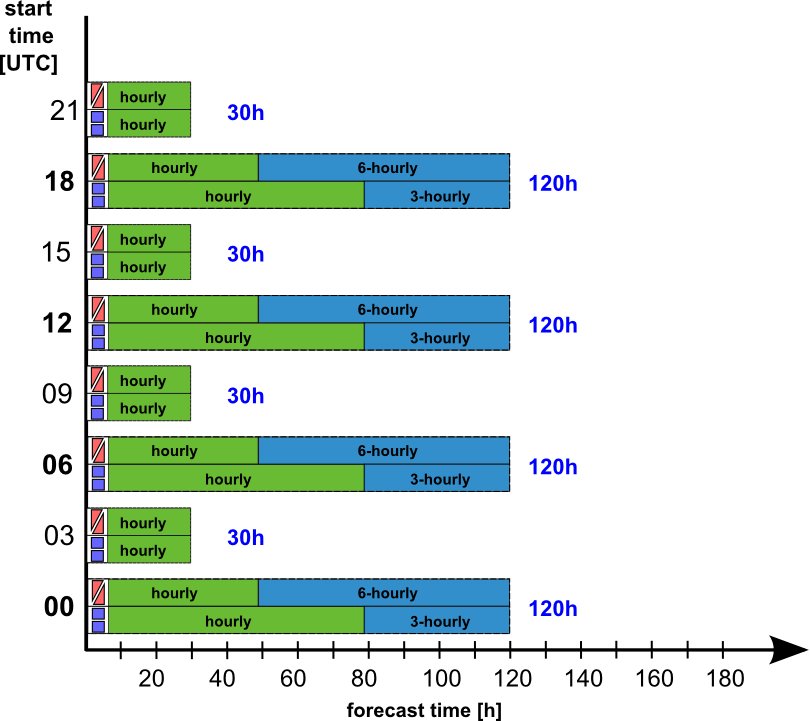
\includegraphics[width=0.92\textwidth]{forecast_length_nest.png}
 \caption{Time span covered by the various EU nest forecasts. A forecast run is launched every three hours.
          Output fields are available hourly up to $VV=78\,\mathrm{h}$ and 3-hourly for larger forecast times. 
          The vertical rules indicate the time until when output is generally available on the native grid 
          (\protect\markRed) and/or on the lat-lon grid (\protect\markBlue). I.e.\ output on the native grid is 
          limited to $VV=48\,\mathrm{h}$.}\label{fig:forecast_length_nest}
\end{figure}

Output is available on two distinct horizontal grids: 
\begin{itemize}
  \item a native triangular grid with an average resolution of $6.5\,\mathrm{km}$, and
  \item a regular latitude-longitude grid with a resolution of $\Delta \lambda = \Delta \Phi=0.0625^{\circ}$.\\
    See Table~\ref{tab:ICON_latlon_summary} for a summary.
\end{itemize}
%
Note that output on the native (triangular) grid is limited to $48\,\mathrm{h}$, whereas output on the regular 
grid is generally available until forecast end. See also Figure \ref{fig:forecast_length_nest}.

Again, in the subsequent tables the availability of specific fields on the native grid ($\,$\markRed$\,$), 
on the lat-lon grid($\,$\markBlue$\,$), or on both grids ($\,$\markRed\markBlue$\,$) is marked in the leftmost column.



% --------------------------------------------------------------------------------
\subsection{Time-constant (external parameter) fields for the EU nest}
% --------------------------------------------------------------------------------

% LaTeX macros that are later used to disable/enable rows in the
% tables of output fields (global/local domain):
\renewcommand{\onlyglb}[1]{}
\renewcommand{\onlyloc}[1]{#1}
%
\begin{vartable}{\caption{Variables exclusively available for $VV=0$ from the forecast databases (\texttt{CAT\_NAME=\$model\_\$run\_\tblu{fc}\_\$suite}, $s[h]=0$)}\label{table:nest:init_output}}

  % --------- include table of variables
  % 
  \groups[tri][]   & CLAT                          &  Geographical latitude of native grid triangle cell center                              &               0                                   &                     191                     &                    1                       &                 1/--                            &                      inst                   &        $\mathrm{Deg.\, N}$   \\
\groups[tri][]   & CLON                          &  Geographical longitude of native grid triangle cell center                             &               0                                   &                     191                     &                    2                       &                 1/--                            &                      inst                   &        $\mathrm{Deg.\, E}$   \\
\groups[tri][]   & ELAT                          &  Geographical latitude of native grid triangle edge midpoint                            &               0                                   &                     191                     &                    1                       &                 1/--                            &                      inst                   &        $\mathrm{Deg.\, N}$   \\
\groups[tri][]   & ELON                          &  Geographical longitude of native grid triangle edge midpoint                           &               0                                   &                     191                     &                    2                       &                 1/--                            &                      inst                   &        $\mathrm{Deg.\, E}$   \\
\groups[tri][]   & VLAT                          &  Geographical latitude of native grid triangle vertex                                   &               0                                   &                     191                     &                    1                       &                 1/--                            &                      inst                   &        $\mathrm{Deg.\, N}$   \\
\groups[tri][]   & VLON                          &  Geographical longitude of native grid triangle vertex                                  &               0                                   &                     191                     &                    2                       &                 1/--                            &                      inst                   &        $\mathrm{Deg.\, E}$   \\
\groups[tri][ll] & DEPTH\_LK                     &  Lake depth                                                                             &               1                                   &                       2                     &                    0                       &                 1/162                           &                      inst                   &        $\mathrm{m}$ \\
\groups[tri][ll] & FR\_LAND                      &  Land fraction (possible range [$0,1$])                                                 &               2                                   &                       0                     &                    0                       &                 1/--                            &                      inst                   &        $1$ \\
\groups[tri][ll] & FR\_LAKE                      &  Fresh water lake fraction (possible range [$0,1$])                                     &               1                                   &                       2                     &                    2                       &                 1/--                            &                      inst                   &        $1$ \\
\groups[tri][ll] & HHL                           &  Geometric height of model half levels above msl                                        &               0                                   &                       3                     &                    6                       &                 150/101                         &                      inst                   &        $\mathrm{m}$   \\
\groups[tri][ll] & HSURF                         &  Geometric height of the earths surface above msl                                       &               0                                   &                       3                     &                    6                       &                 1/101                           &                      inst                   &        $\mathrm{m}$   \\
\groups[tri][ll] & LAI                           &  Leaf area index                                                                        &               2                                   &                       0                     &                   28                       &                 1/--                            &                      inst                   &        $1$ \\
\groups[tri][]   & NDVIRATIO                     &  ratio of current NDVI (normalized differential vegetation index) to annual max         &               2                                   &                       0                     &                  192                       &                 1/--                            &                      inst                   &        $1$ \\
\groups[tri][ll] & PLCOV                         &  Plant cover                                                                            &               2                                   &                       0                     &                    4                       &                 1/--                            &                      inst                   &        $\mathrm{\%}$ \\
\groups[tri][ll] & ROOTDP                        &  Root depth of vegetation                                                               &               2                                   &                       0                     &                   32                       &                 1/--                            &                      inst                   &        $\mathrm{m}$ \\
\groups[tri][ll] & SOILTYP                       &  Soil type of land fraction  (9 types $[1,\dots, 9]$)                                   &               2                                   &                       3                     &                  196                       &                 1/--                            &                      inst                   &        $1$ \\
  % ------------------------------------

\end{vartable}


% --------------------------------------------------------------------------------
\subsection{Multi-level fields on native hybrid vertical levels for the EU nest}
% --------------------------------------------------------------------------------

% LaTeX macros that are later used to disable/enable rows in the
% tables of output fields (global/local domain):
\renewcommand{\onlyglb}[1]{}
\renewcommand{\onlyloc}[1]{#1}
%
\begin{vartable}{\caption{Hybrid multi-level forecast ($VV>0$) and initialised analysis ($VV=0$) products}}
  
  % --------- include table of variables
  % 
  % TABLE OF VV>0 MULTI-LEVEL FIELDS FROM THE FORECAST DATABASE
%
% This file contains the table data for both the GLOBAL and the EU NEST:
%
% table rows that are only part of the GLOBAL  grid output should be enclosed by         \onlyglb{ ... }
% table rows that are only part of the EU NEST grid output should be enclosed by         \onlyloc{ ... }
%
% ADDITIONAL NOTES:
%
% 1. Variables required to drive INT2LM/COSMO-DE are marked by comment "i2l",
%    see "~for1han/const/iglo/namelst.output.i2l"
%    It is used by script build_varlists.py
%
%    > For the EU nest these are the fields required for the native grid. 
% 
%    ml_varlist           = 'U',         'V',         'W',         'T',         'P',
%                           'QV',        'QC',        'QI',        'QR',        'QS',
%                           'W_I',       'T_G',       'QV_S',
%                           'T_SNOW',    'W_SNOW',    'RHO_SNOW',  'FRESHSNW',
%                           'T_SO',      'W_SO',      'H_ICE',     'T_ICE',
\svnInfo $Id$
\\[-0.5em] % without this dummy line, TikZ does not seem to get the marker position right...
%
%
          \groups[\onlyglb{tri}][         ll ] & CLC                        &  Cloud cover                                                                               &               0/6/22                      &                 150/150                         &                      inst        &             &        $\mathrm{\%}$ \\             
\onlyglb{ \groups[tri          ][            ] & DEN                        &  Density of moist air                                                                      &               0/3/10                      &                 150/150                         &                      inst        &     --      &        $\mathrm{kg\,m^{-3}}$ \\     }
          \groups[tri          ][            ] & DTKE\_CON                  &  Buoyancy-production of TKE due to sub grid scale convection                               &               0/19/219                    &                 150/--                          &                      inst        &     --      &        $\mathrm{m^{2}\,s^{-3}}$ \\   
          \groups[tri          ][            ] & DTKE\_HSH                  &  Production of TKE due to horizontal shear                                                 &               0/19/220                    &                 150/--                          &                      inst        &     --      &        $\mathrm{m^{2}\,s^{-3}}$ \\   
          \groups[tri          ][         ll ] & P                          &  Pressure                                                                                  &               0/3/0                       &                 150/150                         &                      inst        &             &        $\mathrm{Pa}$         \\     % i2l 
          \groups[tri          ][         ll ] & QC                         &  \textcolor{red}{Cloud mixing ratio}\footnotemark[3]                                       &               0/1/22                      &                 150/150                         &                      inst        &             &        $\mathrm{kg\,kg^{-1}}$ \\    % i2l
          \groups[tri          ][         ll ] & QI                         &  \textcolor{red}{Cloud ice mixing ratio}\footnotemark[3]                                   &               0/1/82                      &                 150/150                         &                      inst        &             &        $\mathrm{kg\,kg^{-1}}$ \\    % i2l
          \groups[tri          ][            ] & QR                         &  \textcolor{red}{Rain mixing ratio}\footnotemark[3]                                        &               0/1/24                      &                 150/150                         &                      inst        &     --      &        $\mathrm{kg\,kg^{-1}}$ \\    % i2l
          \groups[tri          ][            ] & QS                         &  \textcolor{red}{Snow mixing ratio}\footnotemark[3]                                        &               0/1/25                      &                 150/150                         &                      inst        &     --      &        $\mathrm{kg\,kg^{-1}}$ \\    % i2l 
          \groups[tri          ][         ll ] & QV                         &  Specific humidity                                                                         &               0/1/0                       &                 150/150                         &                      inst        &             &        $\mathrm{kg\,kg^{-1}}$ \\    % i2l
          \groups[tri          ][         ll ] & T                          &  Temperature                                                                               &               0/0/0                       &                 150/150                         &                      inst        &             &        $\mathrm{K}$          \\     % i2l 
          \groups[tri          ][         ll ] & TKE                        &  Turbulent kinetic energy                                                                  &               0/19/11                     &                 150/--                          &                      inst        &             &        $\mathrm{m^{2}\,s^{-2}}$ \\  
          \groups[tri          ][         ll ] & U                          &  Zonal wind                                                                                &               0/2/2                       &                 150/150                         &                      inst        &             &        $\mathrm{m\,s^{-1}}$   \\    % i2l
          \groups[tri          ][         ll ] & V                          &  Meridional wind                                                                           &               0/2/3                       &                 150/150                         &                      inst        &             &        $\mathrm{m\,s^{-1}}$   \\    % i2l
          \groups[tri          ][         ll ] & W                          &  Vertical wind                                                                             &               0/2/9                       &                 150/--                          &                      inst        &             &        $\mathrm{m\,s^{-1}}$   \\    % i2l


  % ------------------------------------
  
\end{vartable}
\footnotetext[2]{for the time being, erroneously encoded as mixing ratios instead of specific quantities}


% --------------------------------------------------------------------------------
\subsection{Multi-level fields interpolated to pressure levels}
% --------------------------------------------------------------------------------

\renewcommand{\new}[1]{\textcolor{red}{#1}}
%
% List of pressure levels taken from COSMO-EU DB documentation, Section 5.1 (2015-03-27)
%
\renewcommand{\pressurelevelsRegular}{$1000$, \new{$975$}, $950$, \new{$925$}, \new{$900$}, 
                                    \new{$875$}, $850$, \new{$825$}, \new{$800$}, 
                                    \new{$775$}, \new{$750$}, \new{$725$}, $700$, $600$, 
                                    $500$, $400$, $300$, $250$, $200$, \new{$150$}, \new{$100$}, 
                                    \new{$70$}, \new{$50$}~$\mathrm{hPa}$}

For regular grid output the following pressure levels are available: 
\begin{center}
\begin{minipage}{0.5\linewidth}
\pressurelevelsRegular. 
\end{minipage}
\end{center}

Newly available pressure levels (as compared to COSMO-EU) are highlighted in red. 
The output fields are listed in Table~\ref{table:nest:output_pressurelevels_regular}.

On the native (triangular) grid no output is generated for pressure levels.

\renewcommand{\new}[1]{#1}

\begin{vartable}{\caption{Regular grid output on the ICON EU Nest:
      Multi-level forecast ($VV>0$) and initialised analysis ($VV=0$) products 
      interpolated to pressure levels \pressurelevelsRegular.}\label{table:nest:output_pressurelevels_regular}}
  
  \groups[][ll] & FI                         &  Geopotential                                                                              &               0                                   &                     3                       &                    4                       &                 100/--                          &                      inst                   &        $\mathrm{m^{2}\,s^{-2}}$   \\ % pl
  \groups[][ll] & OMEGA                      &  Vertical velocity in pressure coordinates ($\omega=\mathrm{d}p/\mathrm{d}t$)              &               0                                   &                     2                       &                    8                       &                 100/--                          &                      inst                   &        $\mathrm{Pa\,s^{-1}}$  \\     % pl
  \groups[][ll] & RELHUM                     &  Relative humidity (with respect to water)                                                 &               0                                   &                     1                       &                    1                       &                 100/--                          &                      inst                   &        $\mathrm{\%}$          \\     % pl
  \groups[][ll] & T                          &  Temperature                                                                               &               0                                   &                     0                       &                    0                       &                 100/--                          &                      inst                   &        $\mathrm{K}$          \\      % pl
  \groups[][ll] & U                          &  Zonal wind                                                                                &               0                                   &                     2                       &                    2                       &                 100/--                          &                      inst                   &        $\mathrm{m\,s^{-1}}$   \\     % pl
  \groups[][ll] & V                          &  Meridional wind                                                                           &               0                                   &                     2                       &                    3                       &                 100/--                          &                      inst                   &        $\mathrm{m\,s^{-1}}$   \\     % pl
  
\end{vartable}



%% --------------------------------------------------------------------------------
%\subsection{Multi-level fields interpolated to height levels}
%% --------------------------------------------------------------------------------
%
%
%%
%% List of pressure levels taken from COSMO-EU DB documentation, Section 5.1 (2015-03-27)
%%
%\renewcommand{\heightlevelsRegular}{$10000$, $5000$, $3000$, $2000$, $1500$, $1000$, $500$, $100$~$\mathrm{m}$}
%
%\begin{vartable}{\caption{Regular grid output on the ICON EU Nest:
%      Multi-level forecast ($VV>0$) and initialised analysis ($VV=0$) products interpolated to height levels \heightlevelsRegular
%      ~(above mean sea level).}\label{table:nest:output_heightlevels_regular}}
%  
%  \groups[][ll] & U                          &  Zonal wind                                                                                &               0                                   &                     2                       &                    2                       &                 102/--                          &                      inst                   &        $\mathrm{m\,s^{-1}}$   \\ % pl
%  \groups[][ll] & V                          &  Meridional wind                                                                           &               0                                   &                     2                       &                    3                       &                 102/--                          &                      inst                   &        $\mathrm{m\,s^{-1}}$   \\ % pl
%  \groups[][ll] & W                          &  Vertical wind                                                                             &               0                                   &                     2                       &                    9                       &                 102/--                          &                      inst                   &        $\mathrm{m\,s^{-1}}$   \\ % pl
%  \groups[][ll] & T                          &  Temperature                                                                               &               0                                   &                     0                       &                    0                       &                 102/--                          &                      inst                   &        $\mathrm{K}$          \\  % pl
%  \groups[][ll] & P                          &  Pressure                                                                                  &               0                                   &                     3                       &                    0                       &                 102/--                          &                      inst                   &        $\mathrm{Pa}$         \\  % pl
%
%\end{vartable}
%


% --------------------------------------------------------------------------------
\subsection{Single-level fields}
% --------------------------------------------------------------------------------

% LaTeX macros that are later used to disable/enable rows in the
% tables of output fields (global/local domain):
\renewcommand{\onlyglb}[1]{}
\renewcommand{\onlyloc}[1]{#1}
%
\begin{vartable}{\caption[]{Single-level forecast ($VV>0$) and initialised analysis ($VV=0$) products on the ICON EU Nest}}

  % --------- include table of variables
  % TABLE OF VV>0 MULTI-LEVEL FIELDS FROM THE FORECAST DATABASE
%
% This file contains the table data for both the GLOBAL and the EU NEST:
%
% table rows that are only part of the GLOBAL  grid output should be enclosed by         \onlyglb{ ... }
% table rows that are only part of the EU NEST grid output should be enclosed by         \onlyloc{ ... }
%
% ADDITIONAL NOTES:
%
% 1. Variables required to drive INT2LM/COSMO-DE are marked by comment "i2l",
%    see "~for1han/const/iglo/namelst.output.i2l"
%    It is used by script build_varlists.py
%
%    > For the EU nest these are the fields required for the native grid. 
% 
%    ml_varlist           = 'U',         'V',         'W',         'T',         'P',
%                           'QV',        'QC',        'QI',        'QR',        'QS',
%                           'W_I',       'T_G',       'QV_S',
%                           'T_SNOW',    'W_SNOW',    'RHO_SNOW',  'FRESHSNW',
%                           'T_SO',      'W_SO',      'H_ICE',     'T_ICE',
%
%
\svnInfo $Id$
\\[-0.5em] % without this dummy line, TikZ does not seem to get the marker position right...
%
%
           \groups[\onlyglb{tri}][         ll ] & ALB\_RAD                       &  Shortwave broadband albedo for diffuse radiation                                      &               0                                   &                    19                       &                     1                      &                 1/--                            &                      inst                   &        $\mathrm{\%}$    \\            
           \groups[\onlyglb{tri}][         ll ] & ALHFL\_S                       &  Latent heat net flux at surface (average since model start)                           &               0                                   &                     0                       &                    10                      &                 1/--                            &                      avg                    &        $\mathrm{W\,m^{-2}}$  \\
           \groups[             ][         ll ] & APAB\_S                        &  Photosynthetically active radiation flux at surface (average since model start)       &               0                                   &                     4                       &                    10                      &                 1/--                            &                      avg                    &        $\mathrm{W\,m^{-2}}$    \\    
           \groups[\onlyglb{tri}][         ll ] & ASHFL\_S                       &  Sensible heat net flux at surface (average since model start)                         &               0                                   &                     0                       &                    11                      &                 1/--                            &                      avg                    &        $\mathrm{W\,m^{-2}}$  \\
           \groups[\onlyglb{tri}][         ll ] & ASOB\_S                        &  Net short-wave radiation flux at surface (average since model start)                  &               0                                   &                     4                       &                     9                      &                 1/--                            &                      avg                    &        $\mathrm{W\,m^{-2}}$    \\    
           \groups[\onlyglb{tri}][         ll ] & ASOB\_T                        &  Net short-wave radiation flux at TOA (average since model start)                      &               0                                   &                     4                       &                     9                      &                 8/--                            &                      avg                    &        $\mathrm{W\,m^{-2}}$    \\    
           \groups[\onlyglb{tri}][         ll ] & ASWDIFD\_S                     &  Surface down solar diffuse radiation (average since model start)                      &               0                                   &                     4                       &                   199                      &                 1/--                            &                      avg                    &        $\mathrm{W\,m^{-2}}$  \\      
           \groups[\onlyglb{tri}][         ll ] & ASWDIFU\_S                     &  Surface up solar diffuse radiation (average since model start)                        &               0                                   &                     4                       &                     8                      &                 1/--                            &                      avg                    &        $\mathrm{W\,m^{-2}}$  \\      
           \groups[\onlyglb{tri}][         ll ] & ASWDIR\_S                      &  Surface down solar direct radiation (average since model start)                       &               0                                   &                     4                       &                   198                      &                 1/--                            &                      avg                    &        $\mathrm{W\,m^{-2}}$  \\      
           \groups[\onlyglb{tri}][         ll ] & ATHB\_S                        &  Net long-wave radiation flux at surface (average since model start)                   &               0                                   &                     5                       &                     5                      &                 1/--                            &                      avg                    &        $\mathrm{W\,m^{-2}}$    \\    
           \groups[\onlyglb{tri}][         ll ] & ATHB\_T                        &  Net long-wave radiation flux at TOA (average since model start)                       &               0                                   &                     5                       &                     5                      &                 8/--                            &                      avg                    &        $\mathrm{W\,m^{-2}}$    \\    
           \groups[\onlyglb{tri}][         ll ] & AUMFL\_S                       &  U-momentum flux at surface $\overline{u^{\prime}w^{\prime}}^{1/2}$ (average since model start)&       0                                   &                     2                       &                    17                      &                 1/--                            &                      avg                    &        $\mathrm{m}$  \\ 
           \groups[\onlyglb{tri}][         ll ] & AVMFL\_S                       &  V-momentum flux at surface $\overline{v^{\prime}w^{\prime}}^{1/2}$ (average since model start)&       0                                   &                     2                       &                    18                      &                 1/--                            &                      avg                    &        $\mathrm{m}$  \\ 
           \groups[\onlyglb{tri}][\onlyloc{ll}] & CAPE\_CON                      &  Convective available potential energy                                                 &               0                                   &                     7                       &                     6                      &                 1/--                            &                      inst                   &        $\mathrm{J\,kg^{-1}}$  \\  
           \groups[\onlyglb{tri}][         ll ] & CLCH                           &  High level clouds                                                                     &               0                                   &                     6                       &                    22                      &                 100/100                         &                      inst                   &        $\mathrm{\%}$          \\    
           \groups[\onlyglb{tri}][         ll ] & CLCM                           &  Mid level clouds                                                                      &               0                                   &                     6                       &                    22                      &                 100/100                         &                      inst                   &        $\mathrm{\%}$          \\    
           \groups[\onlyglb{tri}][         ll ] & CLCL                           &  Low level clouds                                                                      &               0                                   &                     6                       &                    22                      &                 100/1                           &                      inst                   &        $\mathrm{\%}$          \\    
           \groups[\onlyglb{tri}][         ll ] & CLCT                           &  Total cloud cover                                                                     &               0                                   &                     6                       &                     1                      &                 1/--                            &                      inst                   &        $\mathrm{\%}$          \\    
           \groups[             ][         ll ] & CLCT\_MOD                      &  Modified total cloud cover for media                                                  &               0                                   &                     6                       &                   199                      &                 1/--                            &                      inst                   &        $1$                    \\     
           \groups[             ][         ll ] & CLDEPTH                        &  Modified cloud depth for media                                                        &               0                                   &                     6                       &                   198                      &                 1/--                            &                      inst                   &        $1$                    \\     
           \groups[         tri ][            ] & FRESHSNW                       &  Fresh snow factor (weighting function for albedo indicating freshness of snow)        &               0                                   &                     1                       &                   203                      &                 1/--                            &                      inst                   &        $1$  \\                       % i2l
           \groups[         tri ][            ] & FR\_ICE                        &  Sea/lake ice cover  (possible range: $[0,1]$)                                         &              10                                   &                     2                       &                     0                      &                 1/--                            &                      inst                   &        $1$  \\
           \groups[\onlyglb{tri}][         ll ] & HBAS\_CON                      &  Height of convective cloud base above msl                                             &               0                                   &                     6                       &                    26                      &                 2/101                           &                      inst                   &        $\mathrm{m}$  \\              
           \groups[         tri ][         ll ] & H\_ICE                         &  Sea/Lake ice thickness (Max: $3\,\mathrm{m}$)                                         &              10                                   &                     2                       &                     1                      &                 1/--                            &                      inst                   &        $\mathrm{m}$  \\             % i2l
           \groups[\onlyglb{tri}][         ll ] & H\_SNOW                        &  Snow depth                                                                            &               0                                   &                     1                       &                    11                      &                 1/--                            &                      inst                   &        $\mathrm{m}$  \\              
           \groups[\onlyglb{tri}][         ll ] & HTOP\_CON                      &  Height of convective cloud top above msl                                              &               0                                   &                     6                       &                    27                      &                 3/101                           &                      inst                   &        $\mathrm{m}$  \\              
           \groups[\onlyglb{tri}][         ll ] & HTOP\_DC                       &  Height of top of dry convection above msl                                             &               0                                   &                     6                       &                   196                      &                 3/101                           &                      inst                   &        $\mathrm{m}$  \\              
           \groups[\onlyglb{tri}][         ll ] & HZEROCL                        &  Height of 0 degree Celsius isotherm above msl                                         &               0                                   &                     3                       &                     6                      &                 4/101                           &                      inst                   &        $\mathrm{m}$  \\              
           \groups[             ][         ll ] & PMSL                           &  Surface pressure reduced to msl                                                       &               0                                   &                     3                       &                     1                      &                 101/--                          &                      inst                   &        $\mathrm{Pa}$   \\
           \groups[\onlyglb{tri}][         ll ] & PS                             &  Surface pressure (not reduced)                                                        &               0                                   &                     3                       &                    0                       &                 1/--                            &                      inst                   &        $\mathrm{Pa}$   \\            
           \groups[             ][         ll ] & QV\_2M                         &  Specific humidity at 2m above ground                                                  &               0                                   &                     1                       &                     0                      &               103/--                            &                      inst                   &        $\mathrm{kg\,kg^{-1}}$ \\
           \groups[         tri ][         ll ] & QV\_S                          &  Surface specific humidity                                                             &               0                                   &                     1                       &                    0                       &                 1/--                            &                      inst                   &        $\mathrm{kg\,kg^{-1}}$    \\ % i2l 
           \groups[\onlyglb{tri}][         ll ] & RAIN\_CON\onlyglb{\footnotemark[4]} &  Convective rain (accumulated since model start)                                  &               0                                   &                     1                       &                    76                      &                 1/--                            &                      accu                   &        $\mathrm{kg\,m^{-2}}$    \\   
           \groups[\onlyglb{tri}][         ll ] & RAIN\_GSP\onlyglb{\footnotemark[4]} &  Large scale rain (accumulated since model start)                                 &               0                                   &                     1                       &                    77                      &                 1/--                            &                      accu                   &        $\mathrm{kg\,m^{-2}}$    \\   
           \groups[             ][         ll ] & RELHUM\_2M                     &  Relative humidity at 2m above ground                                                  &               0                                   &                     1                       &                     1                      &               103/--                            &                      inst                   &        $\mathrm{\%}$     \\          
           \groups[         tri ][         ll ] & RHO\_SNOW                      &  Snow density                                                                          &               0                                   &                     1                       &                    61                      &                 1/--                            &                      inst                   &        $\mathrm{kg\,m^{-3}}$  \\     % i2l
 \onlyglb{ \groups[         tri ][            ] & RSTOM                          &  Stomatal resistance                                                                   &               2                                   &                     0                       &                   195                      &                 1/--                            &                      inst                   &        $\mathrm{s\,m^{-1}}$  \\     }
           \groups[\onlyglb{tri}][         ll ] & RUNOFF\_G                      &  Soil water runoff (accumulated since model start)                                     &               2                                   &                     0                       &                     5                      &                 106/--                          &                      accu                   &        $\mathrm{kg\,m^{-2}}$  \\                                    
           \groups[\onlyglb{tri}][         ll ] & RUNOFF\_S                      &  Surface water runoff (accumulated since model start)                                  &               2                                   &                     0                       &                     5                      &                 106/--                          &                      accu                   &        $\mathrm{kg\,m^{-2}}$  \\     
           \groups[\onlyglb{tri}][         ll ] & SNOW\_CON\onlyglb{\footnotemark[4]} &  Convective snowfall water equivalent (accumulated since model start)             &               0                                   &                     1                       &                    55                      &                 1/--                            &                      accu                   &        $\mathrm{kg\,m^{-2}}$    \\   
           \groups[\onlyglb{tri}][         ll ] & SNOW\_GSP\onlyglb{\footnotemark[4]} &  Large snowfall water equivalent (accumulated since model start)                  &               0                                   &                     1                       &                    56                      &                 1/--                            &                      accu                   &        $\mathrm{kg\,m^{-2}}$    \\   
 \onlyloc{ \groups[             ][         ll ] & SNOWLMT\footnotemark[5]        &  Height of snowfall limit above MSL                                                    &               0                                   &                     1                       &                   204                      &                 4/101                           &                      inst                   &        $\mathrm{m}$    \\   }
 \onlyglb{ \groups[             ][         ll ] & SOBS\_RAD                      &  Net short-wave radiation flux at surface (instantaneous)                              &               0                                   &                     4                       &                     9                      &                 1/--                            &                      inst                   &        $\mathrm{W\,m^{-2}}$    \\    }
           \groups[\onlyglb{tri}][         ll ] & T\_2M                          &  Temperature at 2m above ground                                                        &               0                                   &                     0                       &                     0                      &               103/--                            &                      inst                   &        $\mathrm{K}$          \\      
           \groups[\onlyglb{tri}][         ll ] & TCH                            &  Turbulent transfer coefficient for heat and moisture (surface)                        &               0                                   &                     0                       &                    19                      &                 1/--                            &                      inst                   &        $1$    \\ 
           \groups[\onlyglb{tri}][         ll ] & TCM                            &  Turbulent transfer coefficient for momentum (surface)                                 &               0                                   &                     2                       &                    29                      &                 1/--                            &                      inst                   &        $1$    \\ 
           \groups[\onlyglb{tri}][         ll ] & TD\_2M                         &  Dew point temperature at 2m above ground                                              &               0                                   &                     0                       &                     6                      &               103/--                            &                      inst                   &        $\mathrm{K}$          \\      
           \groups[         tri ][         ll ] & T\_G                           &  Ground temperature (temperature at sfc-atm interface)                                 &               0                                   &                     0                       &                    0                       &                 1/--                            &                      inst                   &        $\mathrm{K}$    \\           % i2l
 \onlyglb{ \groups[             ][         ll ] & THBS\_RAD                      &  Net long-wave radiation flux at surface (instantaneous)                               &               0                                   &                     5                       &                     5                      &                 1/--                            &                      inst                   &        $\mathrm{W\,m^{-2}}$    \\    }
           \groups[         tri ][         ll ] & T\_ICE                         &  Sea/Lake ice temperature (at ice-atm interface)                                       &              10                                   &                     2                       &                     8                      &                 1/--                            &                      inst                   &        $\mathrm{K}$  \\             % i2l 
           \groups[\onlyglb{tri}][         ll ] & TMAX\_2M                       &  Maximum temperature at 2m above ground                                                &               0                                   &                     0                       &                     0                      &               103/--                            &                      max                    &        $\mathrm{K}$          \\     
           \groups[\onlyglb{tri}][         ll ] & TMIN\_2M                       &  Minimum temperature at 2m above ground                                                &               0                                   &                     0                       &                     0                      &               103/--                            &                      min                    &        $\mathrm{K}$          \\     
           \groups[\onlyglb{tri}][         ll ] & TOT\_PREC\onlyglb{\footnotemark[4]} &  Total precipitation (accumulated since model start)                              &               0                                   &                     1                       &                    52                      &                 1/--                            &                      accu                   &        $\mathrm{kg\,m^{-2}}$  \\     
           \groups[\onlyglb{tri}][         ll ] & TQC                            &  Column integrated cloud water (grid scale)                                            &               0                                   &                     1                       &                    69                      &                 1/--                            &                      inst                   &        $\mathrm{kg\,m^{-2}}$  \\    
 \onlyglb{ \groups[         tri ][         ll ] & TQC\_DIA                       &  Total column integrated cloud water (including sub-grid-scale contribution)           &               0                                   &                     1                       &                   215                      &                 1/--                            &                      inst                   &        $\mathrm{kg\,m^{-2}}$  \\    }
           \groups[\onlyglb{tri}][         ll ] & TQI                            &  Column integrated cloud ice (grid scale)                                              &               0                                   &                     1                       &                    70                      &                 1/--                            &                      inst                   &        $\mathrm{kg\,m^{-2}}$  \\    
 \onlyglb{ \groups[         tri ][         ll ] & TQI\_DIA                       &  Total column integrated cloud ice (including sub-grid-scale contribution)             &               0                                   &                     1                       &                   216                      &                 1/--                            &                      inst                   &        $\mathrm{kg\,m^{-2}}$  \\    }
           \groups[\onlyglb{tri}][         ll ] & TQR                            &  Column integrated rain (grid scale)                                                   &               0                                   &                     1                       &                    45                      &                 1/--                            &                      inst                   &        $\mathrm{kg\,m^{-2}}$  \\
           \groups[\onlyglb{tri}][         ll ] & TQS                            &  Column integrated snow (grid scale)                                                   &               0                                   &                     1                       &                    46                      &                 1/--                            &                      inst                   &        $\mathrm{kg\,m^{-2}}$  \\ 
           \groups[\onlyglb{tri}][         ll ] & TQV                            &  Column integrated water vapour (grid scale)                                           &               0                                   &                     1                       &                    64                      &                 1/--                            &                      inst                   &        $\mathrm{kg\,m^{-2}}$  \\    
           \groups[\onlyglb{tri}][\onlyloc{ll}] & T\_S                           &  Temperature of the soil surface (equivalent to T\_SO(0))                              &               2                                   &                     3                       &                    18                      &                 1/--                            &                      inst                   &        $\mathrm{K}$    \\             
           \groups[         tri ][         ll ] & T\_SNOW                        &  Temperature of the snow surface                                                       &               0                                   &                     0                       &                    18                      &                 1/--                            &                      inst                   &        $\mathrm{K}$    \\            % i2l
           \groups[\onlyglb{tri}][         ll ] & U\_10M                         &  Zonal wind at 10m above ground                                                        &               0                                   &                     2                       &                     2                      &               103/--                            &                      inst                   &        $\mathrm{m\,s^{-1}}$  \\      
           \groups[\onlyglb{tri}][         ll ] & V\_10M                         &  Meridional wind at 10m above ground                                                   &               0                                   &                     2                       &                     3                      &               103/--                            &                      inst                   &        $\mathrm{m\,s^{-1}}$  \\      
           \groups[\onlyglb{tri}][         ll ] & VMAX\_10M                      &  Maximum wind at $10\,\mathrm{m}$ above ground                                         &               0                                   &                     2                       &                    22                      &               103/--                            &                      max                    &        $\mathrm{m\,s^{-1}}$   \\     
           \groups[         tri ][            ] & W\_I                           &  Plant canopy surface water                                                            &               2                                   &                     0                       &                    13                      &                 1/--                            &                      inst                   &        $\mathrm{kg\,m^{-2}}$    \\ % i2l
           \groups[         tri ][         ll ] & W\_SNOW                        &  Snow depth water equivalent                                                           &               0                                   &                     1                       &                    60                      &                 1/--                            &                      inst                   &        $\mathrm{kg\,m^{-2}}$    \\    % i2l
           \groups[\onlyglb{tri}][         ll ] & WW                             &  Weather interpretation  (WMO)                                                         &               0                                   &                    19                       &                    25                      &                 1/--                            &                      inst                   &        $1$ \\                        
           \groups[\onlyglb{tri}][         ll ] & Z0                             &  Surface roughness (above land and water)                                              &               2                                   &                     0                       &                     1                      &                 1/--                            &                      inst                   &        $\mathrm{m}$          \\      

  % ------------------------------------

\end{vartable}

\footnotetext[5]{T\_S is identical to T\_SO at level 0. It will no longer be available in the future. Use T\_SO(0) instead of T\_S.} 


% --------------------------------------------------------------------------------
\subsection{Soil-specific multi-level fields}
% --------------------------------------------------------------------------------


%    Variables required to drive INT2LM/COSMO-DE,
%    see "~for1han/const/iglo/namelst.output.i2l"
%
%    > For the EU nest these are the fields required for the native grid. 
% 
%      'T_SO',      'W_SO'

\begin{vartable}{\caption[]{Multi-level forecast ($VV>0$) and initialised analysis ($VV=0$) products of the soil model}}

  \groups[tri][ll] & T\_SO                          &  Soil temperature                                                                      &               2                                   &                     3                       &                    18                       &               106/--                           &                      inst                   &        $\mathrm{K}$   \\           % i2l
  \groups[tri][ll] & W\_SO                          &  Soil moisture integrated over individual soil layers  (ice + liquid)                  &               2                                   &                     3                       &                    20                       &               106/106                          &                      inst                   &        $\mathrm{kg\,m^{-2}}$   \\  % i2l
  \groups[tri][ll] & W\_SO\_ICE                     &  Soil ice content integrated over individual soil layers                               &               2                                   &                     3                       &                    22                       &               106/106                          &                      inst                   &        $\mathrm{kg\,m^{-2}}$   \\
  
\end{vartable}

Soil temperature is defined at the soil depths given in Table \ref{table:nest:soillayer} (column 2). Levels $1$ to $8$ define the full levels of the soil model. A zero gradient 
condition is assumed between levels $0$ and $1$, meaning that temperatures at the surface-atmosphere interface are set equal to the temperature at the first full level depth.
($0.5\,\mathrm{cm}$). Temperatures are prognosed for layers $1$ to $7$. At the lowermost layer (mid-level height $1458\,\mathrm{cm}$) the temperature is fixed 
to the climatological average $2\,\mathrm{m}$-temperature.

Soil moisture \texttt{W\_SO} is prognosed for layers $1$ to $6$. In the two lowermost layers \texttt{W\_SO} is filled with \texttt{W\_SO(6)} (zero gradient condition).
\begin{table}[H]
\center
\caption{Soil model: vertical distribution of levels and layers}\label{table:nest:soillayer}
 \begin{tabular}{>{\centering\arraybackslash}p{2.0cm}>{\centering\arraybackslash}p{2.5cm}|>{\centering\arraybackslash}p{2.5cm}>{\centering\arraybackslash}p{5.0cm}}
 \toprule
  \bf{level no.}       &  \bf{depth [cm]}        &   \bf{layer no.}        & \bf{upper/lower bounds [cm]} \\
 \midrule
         0             &     $0.0$               &                         &                                     \\
         1             &     $0.5$               &         1               &     $0.0$\, \textemdash\, $1.0$     \\
         2             &     $2.0$               &         2               &     $1.0$\, \textemdash\, $3.0$     \\
         3             &     $6.0$               &         3               &     $3.0$\, \textemdash\, $9.0$     \\
         4             &     $18.0$              &         4               &     $9.0$\, \textemdash\, $27.0$    \\
         5             &     $54.0$              &         5               &    $27.0$\, \textemdash\, $81.0$    \\
         6             &     $162.0$             &         6               &    $81.0$\, \textemdash\, $243.0$   \\
         7             &     $486.0$             &         7               &   $243.0$\, \textemdash\, $729.0$   \\
         8             &     $1458.0$            &         8               &   $729.0$\, \textemdash\, $2187.0$  \\
 \bottomrule
 \end{tabular}
\end{table}




% --------------------------------------------------------------------------------
\subsection{Lake-specific single-level fields}
% --------------------------------------------------------------------------------


%\begin{vartable}{\caption[]{Initialised analysis ($VV=0$) products of the lake model model on the ICON EU nest.}}

%  \groups[tri][  ] & C\_T\_LK                       &  Shape factor with respect to the temperature profile in the thermocline               &               1                                   &                     2                       &                    10                       &               162/166                          &                      inst                   &        $1$    \\
%  \groups[tri][  ] & H\_ML\_LK                      &  Mixed-layer depth                                                                     &               1                                   &                     2                       &                     0                       &                 1/166                          &                      inst                   &        $\mathrm{m}$ \\
%  \groups[tri][  ] & T\_BOT\_LK                     &  Temperature at the water-bottom sediment interface                                    &               1                                   &                     2                       &                     1                       &               162/--                           &                      inst                   &        $\mathrm{K}$ \\
%  \groups[tri][  ] & T\_MNW\_LK                     &  Mean temperature of the water column                                                  &               1                                   &                     2                       &                     1                       &                 1/162                          &                      inst                   &        $\mathrm{K}$ \\
%  \groups[tri][  ] & T\_WML\_LK                     &  Mixed-layer temperature                                                               &               1                                   &                     2                       &                     1                       &                 1/166                          &                      inst                   &        $\mathrm{K}$ \\

%\end{vartable}


\begin{vartable}{\caption[]{Single-level forecast ($VV>0$) and initialised analysis ($VV=0$) products of the lake model model on the ICON EU nest.}}

  \groups[tri][] & C\_T\_LK                       &  Shape factor with respect to the temperature profile in the thermocline               &               1                                   &                     2                       &                    10                       &               162/166                          &                      inst                   &        $1$    \\
  \groups[tri][] & H\_ML\_LK                      &  Mixed-layer depth                                                                     &               1                                   &                     2                       &                     0                       &                 1/166                          &                      inst                   &        $\mathrm{m}$ \\
  \groups[tri][] & T\_BOT\_LK                     &  Temperature at the water-bottom sediment interface                                    &               1                                   &                     2                       &                     1                       &               162/--                           &                      inst                   &        $\mathrm{K}$ \\
  \groups[tri][] & T\_MNW\_LK                     &  Mean temperature of the water column                                                  &               1                                   &                     2                       &                     1                       &                 1/162                          &                      inst                   &        $\mathrm{K}$ \\
  \groups[tri][] & T\_WML\_LK                     &  Mixed-layer temperature                                                               &               1                                   &                     2                       &                     1                       &                 1/166                          &                      inst                   &        $\mathrm{K}$ \\
  
\end{vartable}
